%!TEX root = ../report.tex

% 
% Related work
% 


\section{Related Work (~17pgs)}
\label{sec:related_work}
%%!TEX root = ../../report.tex

\subsection{Template} % (fold)
\label{sub:Template}


% Example citation:
THIS IS A CITATION\cite{Braem2013a}
  
The related work section will highly volatile, and will mostly depend on your kind of thesis. Talk with your supervisor in order to know how to write this part. Don't take the following bullet points as a certain truth.

\begin{itemize}
  \item Most important part of the document. Might be divided in 2/3 subsections.
  \item Might be devised into related work and 
  \item Should cite a wide range of references ~30, search in google, google scholar, mendley, IEEE explorer etc..
  \item Summarized table of solutions.
\end{itemize}

Citations should be mostly :
\begin{itemize}
  \item magazine articles
  \item conferences / workshops
  \item books and technical reports
\end{itemize}
And make sure that your citations follow the following criteria:
\begin{itemize}
  \item Conferences: name and year
  \item workshops: name of the workshop, name of the conference, location and year
  \item Magazines: volume, issue (if possible article pages), publisher.
  \item Books: title, publisher, ISBN, year
\end{itemize}
Websites should be added as footnotes~\footnote{www.google.com}

% Example image:
\begin{figure}[hb!]
  \centering
  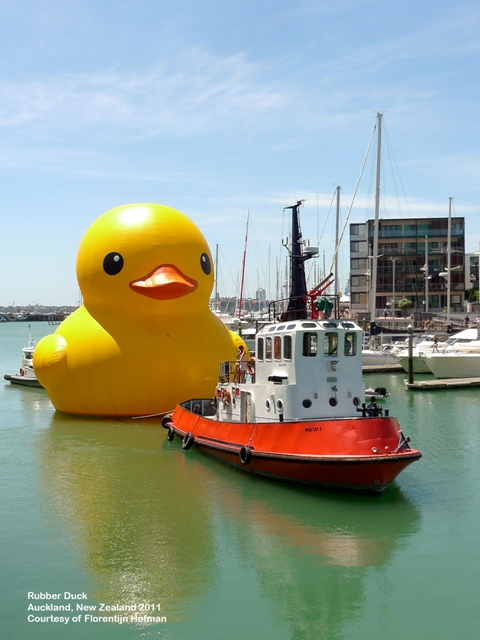
\includegraphics[width=0.95\textwidth]{img/rubberduck.jpg}
  \caption{caption}
  \label{fig:label}
\end{figure}


% subsection Template (end)

As an active research field, there is a lot of work being done in this area. In this section I give an overview of the related work that has been carried out on procedural generation of cities. The generation of cities can be viewd as the sum of a few parts. The generation of terrains, road networks, buildings and other man made structures and cities in general.

The first step, the \emph{generation of terrains} is often left out of procedural generation of cities, because there is also lot of research focused only on this area, mainly to produce models of nature. In this work I will not evaluate specificaly this factor but make specific comments when relevant.

The \emph{road network} is a fundamental step for the generation of any city. It gives the city it's structure and defines the overall look. Most of the road networks are much different from each others and this makes the generalization dificult, but we can see some patterns when we analyze a road network from real cities. And this patterns are important for us if we want to have procedures that mimic this complex patterns. Some cities a have tightly structured grid network, like New York or a concentric radial pattern like Paris and others are purelly organic with the network presenting a nearlly random pattern. And we also have all the shades of grey in between.

Next step is the \emph{generation of building}. This is also not easy, since that there is no limit to the number of different buildings that can be modeled. Since buildings naturally are different from each other both in functionality and style, this is a complex problem to model. One widelly adopted solution is to use group buildings by functionality. The most common groups are \emph{Commercial}, \emph{Residential} and \emph{Industrial} buildings. After this we have to care only about modelling different styles adapted to each functional group. This part is also hard because this ``style'' can be anything. The architectural styles, as explained in the Section~\ref{sub:architectural_styles}, have influences from a lot of different sources. 

The last step is about the generation of the city itself, mainly join all the problems stated above and find a realistic layout for the city and also the generation of the ornamentations for the city like trees and parks. Where to put each building is an important question that can have big impacts in the overall look of the models. Also how to group buildings and create neighborhoods, the function of the building is crucial, industrial buildings usualy are far from the residential ones, the same way that the comercial buildings are close together and also close to the residential areas.

%!TEX root = ../../report.tex
\subsection{CityEngine \cite{Parish2001} \cite{Muller2006}}

It's a three-dimensional (3D) modeling software developed by Procedural Inc. (now part of the Esri R&D Center). It's specialized in the generation of 3D urban environments. With the procedural modeling approach, CityEngine enables an efficient creation of detailed and large-scale 3D city models with a lot of control from the user. 

\subsubsection{RoadNetwork} % (fold)
\label{ssub:roadnetwork1}


The first part to procedurally generate a city is to create a road network to become a backbone of the city and provide an overall structure. For that, CityEngine receives as input maps such as land-water boundaries and population
density. From that input a network of highways is created to connect the areas off high density population, and small roads connect to the highways.
This growth process continues until the average area of each lot is the desired one. The system have a default value, bat it can be set by the user to a different one.

To implement this growth process, it's used an L-System, that computes the road network.


\begin{figure}[htbp]
  \centering
  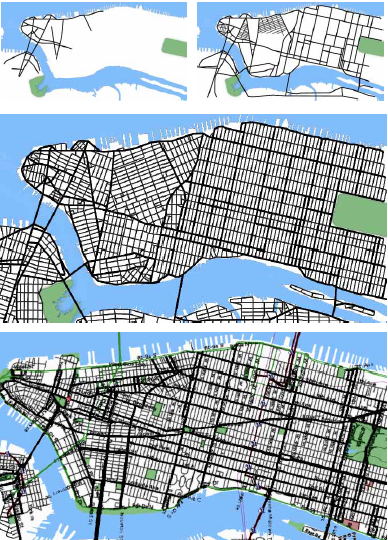
\includegraphics[width=0.5\textwidth]{img/Procedural-Modeling-of-Cities/Capturar.png}
  \caption{Road Map growth}
  \label{fig:city}
\end{figure}

The Figure~\ref{fig:city} shows the evolution of this process in a map of Manhattan. The first two on the top shows the process in different phases during the process, the middle line is the result of the process and the bottom line is the real map of Manhattan for comparison.

% subsubsection roadnetwork (end)Road Network

\subsubsection{Buildings} % (fold)
\label{ssub:buildings1}

To implement the generation of buildings, they created the CGA Shape.

CGA Shape is a Shape Grammar that was introduced by Pascal Muller, Peter Wonka and others, in a paper called ``Procedural Modeling of Buildings''\cite{Parish2001}. It is defined as ``a novel shape grammar for the procedural modelling of CG architecture, produces building shells with high visual quality and geometric detail." To do so, this grammar uses a group of well defined production rules.

This tool allows the user to model buildings with an high control and in different ways. It can be done by text, writing production rules from a shape grammar or with a visual language like Grasshopper 3D, that is nice for simple works but it's impossible to work with a slightly more complex work. 

Mass Modeling
To model a building the first step is to create a mass model of the entire building by assembling basic shapes. With scaling, translation rotation and split applied to basic shapes namely I, L, H, U and T as shown in the Figure~\ref{fig:}.

\begin{figure}[htbp]
  \centering
  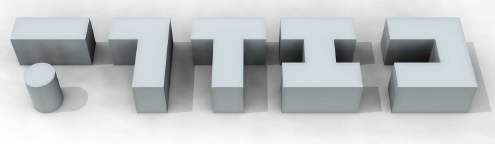
\includegraphics[width=0.95\textwidth]{img/Procedural-Modeling-of-Cities/MassModeling2.png}
  \caption{caption}
  \label{fig:label}
\end{figure}

The next step is to add the roof, from a set of basic roof shapes or general L-Systems.

After that, with the application of the grammar rules in the created mass, it's possible to create complexity to the level that is desired, being able to produce high complex buildings like the one in the following picture.

% subsubsection buildings (end)

\subsubsection{Cities} % (fold)
\label{ssub:Cities1}

The result can be an city like Figure~\ref{fig:bigCity}, with approximately 26000 buildings.

\begin{figure}[htbp]
  \centering
  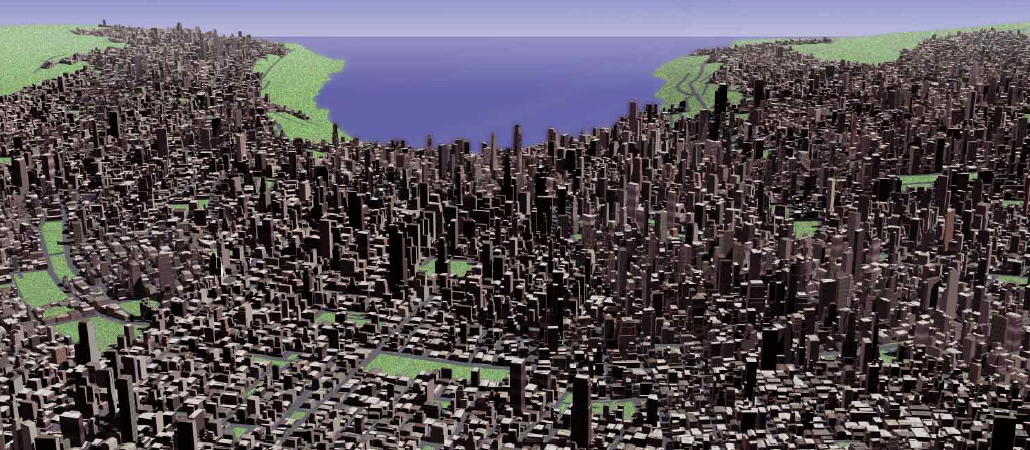
\includegraphics[width=0.95\textwidth]{img/Procedural-Modeling-of-Cities/City.png}
  \caption{City with approximately 26000 buildings.}
  \label{fig:bigCity}
\end{figure}

City Engine results can be imported by Maya, to achieve better results. Like the Figure~\ref{fig:cityMaya}, that represents a ‘virtual’ Manhattan.

\begin{figure}[htbp]
  \centering
  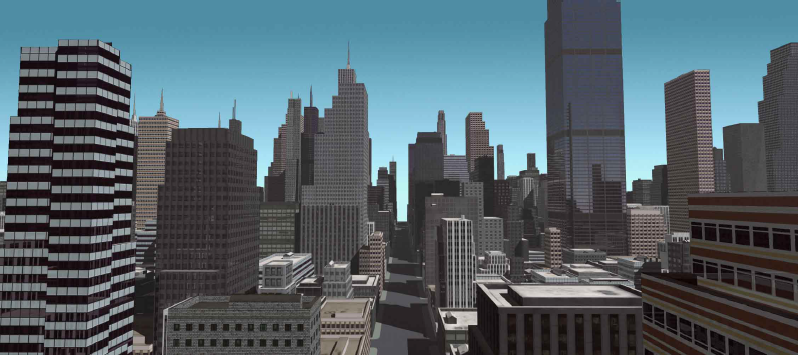
\includegraphics[width=0.95\textwidth]{img/Procedural-Modeling-of-Cities/City_Maya.png}
  \caption{City rendered with Maya.}
  \label{fig:cityMaya}
\end{figure}

% subsubsection subsubsection_name (end)


%!TEX root = ../../report.tex

\subsection{Undiscovered City} % (fold)
\label{sub:undiscovered_city}

In \cite{Greuter2003} Stefan Greuter et al. presented a system that generates in Real-time pseudo infinite virtual cities which can be interactively explored from a first person perspective. In their approach ``all geometrical components of the city are generated as they are encountered by the user." As shown in the Figure~\ref{fig:viewingRange} only the part of city that is inside the viewing range is generate.

\begin{figure}[htbp]
	\centering
	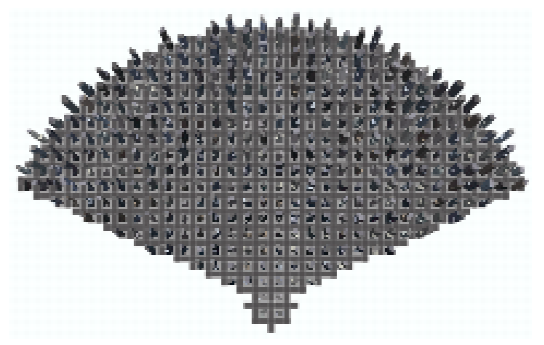
\includegraphics[width=0.85\textwidth]{img/Real-Time-procedural-generation/viewing-range.png}
	\caption{Viewing Range}
	\label{fig:viewingRange}
\end{figure}

\subsubsection{Road Network} % (fold)
\label{ssub:road_network}

The system uses a 2D grid that divide the terrain into square cells. The cells represent proxies for the content that will be procedurally generated. Before the content of each cell is generated, the potential visibility of it is tested, and after that, only the visible cells are filled with content.

After that the roads are created in a uniform grid pattern. This grid does not feel very natural, and in the continuation of the work, this system evolved into a more realistic one with the join of some of the grids to create a less uniform distribution of the buildings.

% subsubsection road_network (end)

\subsubsection{Buildings} % (fold)
\label{ssub:buildings}


To compute the form and appearance of each building, it is used a ``single 32 bit pseudo random number generator seed. The random sequence determines building properties such as width, height and number of floors."
Similar sequences of number result in similar buildings. To avoid that, it is used a a hash function to convert each cell position into a seed.

To generate a building is first is generated a floor plan. To do so, it's randomly selected and merged a set of regular polygons and rectangles, then this is extruded. This is an iterative process, that creates sections from the top to the bottom, by adding more shapes to the the initial shape and extruding as shown in the Figure~\ref{fig:buildings}. Starting from the left, first there is a simple polygon, that is merged with a rectangle and after extrusion, forms the first block that will be the top of the building. After that, another extrusion is made to generate the next block followed by the merge of a rectangle to the floor shape and the generation of a new block and so on.

\begin{figure}[htbp]
	\centering
	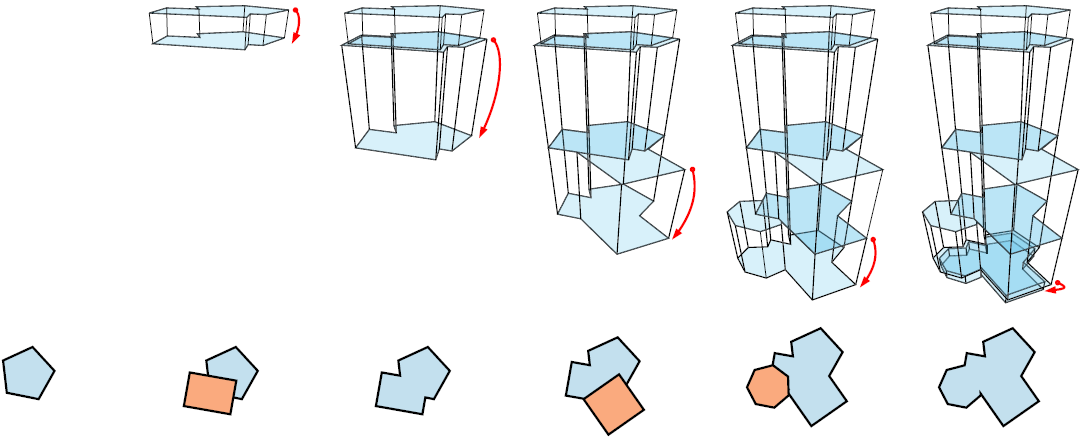
\includegraphics[width=0.85\textwidth]{img/Real-Time-procedural-generation/Building-Generation.png}
	\caption{buildings}
	\label{fig:label}
\end{figure}

With the application of this method very complex architectural forms can be generated, depending only on which forms are selected and the order that is used to merge them.

% subsubsection buildings (end)

% subsection undiscovered_city (end)

%!TEX root = ../../report.tex

\subsection{CityGen } % (fold)
\label{sec:citygen}

CityGen \cite{Kelly2008} it's an interactive system that aims  to ``rapidly create the urban geometry typical of a modern city". The users can interact and control the generation process. The system, like others, is able to generate road networks that act as foundations to the model. It also can generate buildings but can not achieve the complexity and realism of other systems.

\subsubsection{Road Network} % (fold)
\label{ssub:road_network}

CityGen divided this problem in two steps. First the generation of the \emph{Primary Road Network}, and after that, the \emph{Secondary Road Network}. This two steps use different methods to generate the roads.
Undirected planar graphs are used to represent all roads. Two graphs for the Primary roads and one for each zone to store the secondary roads.

\begin{itemize}
	\item[Primary Road Generation] The primary road network uses two graphs, one high level graph that correspond directly to the primary road intersections. It represents the topological structure of the city by it's primary roads, and connections between them. The user is allowed to manipulate this high level graph, to change the high level structure ("topography of the primary road network") of the city .

There is also the low level graph that is generated from the other one, and defines the real path that the roads have in the terrain. It have the same nodes as the first graph and many more, that indicate the points on the terrain which the road passes.

To generate the low level graph it is used ``sampling, plotting and interpolation processes".
\end{itemize}

\begin{figure}[htbp]
	\centering
	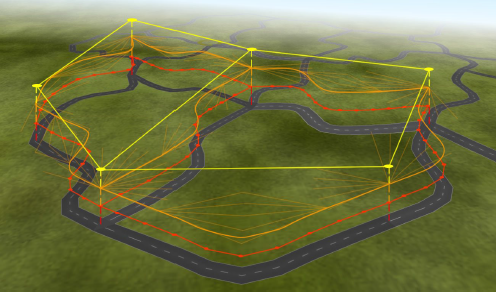
\includegraphics[width=0.85\textwidth]{img/CityGen/RoadGraphs.png}
	\caption{The lighter graph is the High level graph, and the evolution to the darker Low-level graph }
	\label{fig:graphs}
\end{figure}

\begin{itemize}
	\item[Secondary Road Generation] The author defined city cells as districts, that are the areas of terrain that are enclosed by primary roads. The secondary road network is generated inside this cells using a growth based algorithm similar to the L-Systems technique as shown in Figure~\ref{fig:graphs2}.
\end{itemize}


\begin{figure}[htbp]
	\centering
	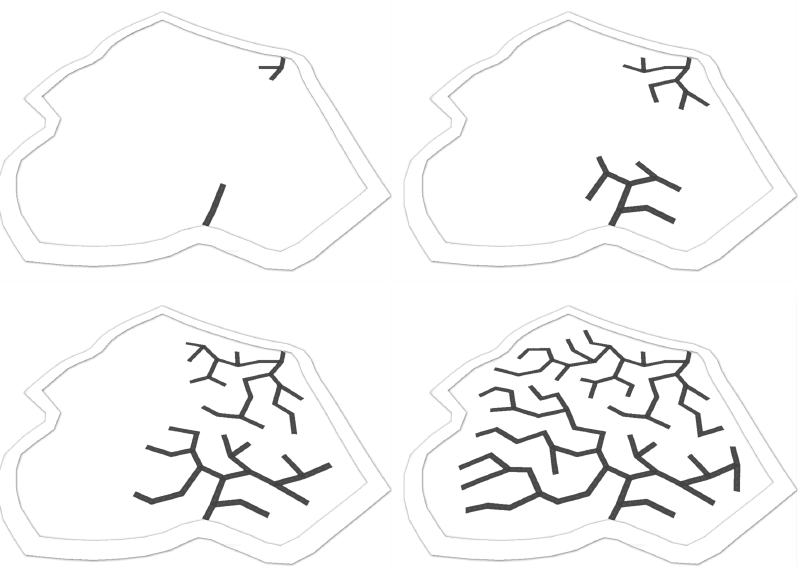
\includegraphics[width=0.85\textwidth]{img/CityGen/SecondaryRoadGrowth.png}
	\caption{}
	\label{fig:graphs2}
\end{figure}

% subsubsection road_network (end)

\subsubsection{Buildings} % (fold)
\label{ssub:buildings}

This system generates buildings also. Each building is created in lots that are identified after the extraction of enclosed regions, called blocks, from the secondary graph. Lots that don't have direct access to the roads are excluded.

Based on the type of block the building footprints are created. After that building geometry is generated by extruding the footprint. The height of each is determined by a height parameter and a noise factor that can be also manipulated. A block is shown in the Figure~\ref{fig:primitiveShapes}, with only primitive shapes.

\begin{figure}[htbp]
	\centering
	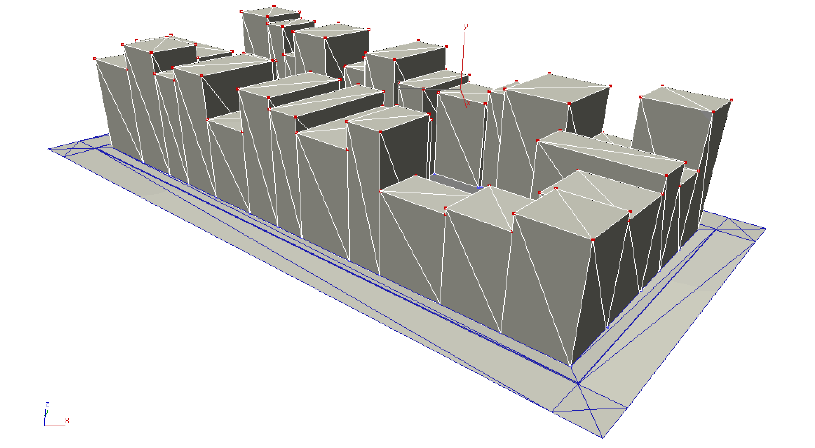
\includegraphics[width=0.85\textwidth]{img/CityGen/BockPrimitiveShapes.png}
	\caption{Primitive Shape Buildings}
	\label{fig:primitiveShapes}
\end{figure}

With this primitive shapes, CityGen uses ``advanced materials with shaders to simulate additional geometry".

% subsubsection buildings (end)

% subsection citygen (end)


%!TEX root = ../../report.tex

\subsection{Inverse Design [NOT DONE]} % (fold)
\label{sub:inverse_design}


In \cite{Vanegas2009} it is presented a different solution from the others already presented.
It's described a framework that enables high level control of the modelling process. It ``provides a mechanism to interactively edit urban models". They apply inverse design to solve the problem of output control. From an existing model, the user can specify high level indicators that describe the desired output and the system change the underlying rules and parameters to get the result as close as possible to the desired.
As the Figure~\ref{fig:loop} shows, the user can change the ``low level" parameters and the ``high level" indicators to control the final output of the system.

\begin{figure}[htbp]
	\centering
	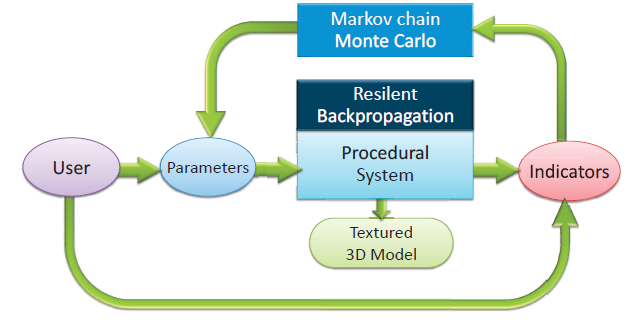
\includegraphics[width=0.95\textwidth]{img/Inverse_Design/TheLoop.PNG}
	\caption{System Pipeline \cite{Vanegas2009}}
	\label{fig:loop}
\end{figure}

This framework uses the indicators as a goal to optimize the parameters. To calculate the values for the parameters they used a version of Monte Carlo Markov Chains (or MCMC) and Resilient Back Propagation.


They implemented a urban procedural engine ``similar to previous city-level procedural modelling work". It was inspired by urban planners, that use the place types concept to represent coherent design patterns of buildings and streets. 


With this approach, the authors claim two main advantages, \emph{Abstraction} and \emph{Interactivity}. They argue that this solution allows urban planners and designers to work at a high level of abstraction, enabling users to manipulate place types, parameters and indicators to create the 3D model they want without wasting time with low level tasks as implementation of low level rules or parameter tuning.
At the same time this approach enables the users to interactively manipulate very complex indicator targets with a ``sophisticated enough" methodology to map target indicators to input low level parameters.


With their teilored version of MCMC and back-propagation they are able to support complex indicators ``enabling control beyond global shape, sush as by high-level semantics and indicators'', and by considering the procedural model as a black box there aren't any limitations to the used grammar.


% \subsubsection{Overview} % (fold)
% \label{ssub:overview}

% A system $P$ produces a geometry $G$ based on \emph{m} input parameter values $\Phi = \{\phi_1,\dots,\phi_m\}$ that is evaluated by an indicator measurement system $I$ which produces a set $\Gamma = \{\gamma_1,\dots,\gama_n\}$ of \emph{n} indicator values.


% % subsubsection overview (end)


% \subsubsection{Inverse Design} % (fold)
% \label{ssub:inverse_design}

% $\Gamma$ - Indicator Values

% $\Phi$ - Input Parameters

% $\Gamma*$ - Target Indicator Values

% $\Phi*$ - Target Parameter Values (specification is optional)


% % subsubsection inverse_design (end)


% \subsubsection{Urban Procedural Model} % (fold)
% \label{ssub:urban_procedural_model}



% subsubsection urban_procedural_model (end)


(\dots)

% subsection inverse_design (end)


%!TEX root = ../../report.tex

\subsection{CityBuilder} % (fold)
\label{sub:citybuilder}


CityBuilder is a system introduced by Watson et. al in \cite{Lechner2003} and \cite{Report2004} ``Procedural City Modeling" and ``Procedural Modeling of Land Use in Cities"}. 
It aims to be self automated to minimize necessary input, only needs the terrain description. Although it allows some other input from the user to give some interaction and control. 
To achieve that, it uses agent based simulation to create a system of agents and behaviours that can model specific entities of a city as developers, planning authorities and road builders. The set of rules for each agent is small to achieve a simple behaviour. With that, they what to make their ``model extendible not only in regard to the types of structures that are produced but also in describing the social and cultural influences prevalent in all cities."

\subsubsection{Road Network} % (fold)
\label{ssub:road_network}
The road network is designed by the agents based on the input terrain description wish will describe the height map and forbidden areas for roads, as water. 
The user can specify that the roads must follow a pre-established gridded pattern, or give the freedom to network to grow more organic. The image presents this two options and a combination of the two with a centre with a gridded pattern ant organic surroundings.


There are two types of road building agents, the extenders and the connectors.

The extenders search the area around exiting developments to look for areas that are not being served by any road to expand the current road network.

The connectors roam trough existing roads and sampling random points in the road network within a given radius. It tries to reach that point trough the road via a BSF. If it cannot reach or the distance needed is over a threshold value, the agent tries to create a road between these two points.


% subsubsection road_network (end)

\subsubsection{Buildings} % (fold)
\label{ssub:buildings}

This system does not develop buildings, but it's developer agents generate parcels and specify the use of the land. They can identify ``at least nine different types of land usages". They perform the role of urban developers that buy land, request planing permission, build and sell. They track the usage of their lands and specify the parameters to the buildings that can be build there.

% subsubsection buildings (end)

\subsubsection{The City} % (fold)
\label{ssub:the_city}

This system develop an evolving conceptual model of one city, that can represent the growth and evolution of a city through the time. 

% subsubsection the_city (end)

% subsection citybuilder (end)


%!TEX root = ../../report.tex

Building Envelopes
\subsection{Building Envelopes [NOT DONE]} % (fold)
\label{sub:building_envelopes}

Sabri Gokmen in \cite{Gokmen2013} presents a way to create envelope systems for buildings. In this case he had a approach that was inspired in Gotheam morphology and leaf venetian patterns.

This article explains form as described by Johann Wolfgang von Goethe in the late eighteenth century. He started by working on annual plants through the work of Linneaus. Goethe considered the external properties of plants to be the result of an internal principle, idea that was influenced by the prior topological work by Linneaus that classified plants according to their physical characteristics.
For Goethe this external properties are not constant and change over time according to environmental conditions.

Forms in architecture are described as a ``topological entity following an overall schema or as a replication of an exiting type that appears fixed (Garcia, 2010)". It says that architects often work with topologies for various buildings and variations are achieved using topological operations. Adding to this is the idea of parametric design to create ``smooth variable systems". This parametric  top-down systems are able to control the overall behaviour of design and have been used to evaluate and adapt performance based approaches in design solutions. ``However this systems are However these systems are ineffective to provide a morphogenetic approach towards design."

Because morphology considers form as the result of a bottom-up process, it is a better method to model growth. Because the form is not defined from start and is the result of the growth process.

Goethe mixed this two ideas namely performance based and morphogenetic approaches. The parametric property is not throughout the system but applied in parts that grow with a morphogenetic approach.

Leaf venetian patterns:
There isn't one certain theory about the guiding principles that support the leaf patterns, there are many theories that try to explain it. One of them is called canalization theory that observes this patterns really as a distribution network, so it depends on the concentration/distributions of auxin producers to efficiently distribute auxin throughout the plant.

Computation of leaf venetian patterns:
The growth algorithm that is presented in this paper is based on the canalization theory. It starts by generating a density map that guides de distribution of auxin sources, that is the second step.
Finally it generates the leaf venetian patterns from the auxin source map.

The generation of the venetian patterns starts by setting root nodes that will be the points from which the patterns will start growing. Then ``at each time step the closest vein node to each auxin source will be defined. Then these nodes will grow towards the average direction influenced by the auxin sources".


% subsection building_envelopes (end)


%!TEX root = ../../report.tex

\subsection{Scene City:} % (fold)
\label{sub:Scene City}

\cite{SceneCity2014}


Scene City is an addon for the 3d application Blender.


“It varies the colors, materials and procedural elements enough to produce a reasonable approximation of a city at a distance, but realism is not a goal, and it does not operate on real data at all.” (http://vterrain.org/Culture/BldCity/Proc/ )

% subsection suicidator_city_generator_ (end)

\subsection{ghostTown:} % (fold)
\label{sub:ghosttown}

http://kilad.net/site/
http://www.kilad.net/GTForum/


It’s a script plugin for 3DS Max from Autodesk.
“Ghost Town is a script that procedurally generates cities and urban environments in only a few clicks, and features a number of options. Such as low or high poly buildings, road layouts, vehicles, trees, facades and an easy to use material and texture system.” (http://cgi.tutsplus.com/tutorials/create-a-detailed-city-with-3d-studio-max-ghost-town--cg-10090)

% subsection ghosttown_ (end)

\subsection{Skyscraper:} % (fold)
\label{sub:skyscraper}

http://www.skyscrapersim.com/index.shtml
Standalone


“Skyscraper aims to be a fully-featured, modular, 3D realtime building simulator, powered by the Scalable Building Simulator (SBS) engine. The main feature SBS provides is a very elaborate and realistic elevator simulator, but also simulates general building features such as walls, floors, stairs, shaftwork and more. Many more things are planned, including gaming support (single and network multiplayer), and a graphical building designer. Skyscraper is written in C++ and uses the OGRE graphics engine, Bullet for collisions and physics, FMOD for sound, the wxWidgets GUI library, and is multiplatform. The current versions aim for a future 2.0 release.” from the official site.

% subsection skyscraper (end)

\subsection{Blended Cities:} % (fold)
\label{sub:blended_cities}

http://jerome.le.chat.free.fr/index.php/en/city-engine/
Addon for Blender

“Blended Cities is an open-source city generator for Blender. it allows to create quickly a large amount of streets and buildings, with various shapes. B.C. fights against squared things : curved streets and odd or cylindric buildings can be created simply, so you can create old towns, not only modern cities.”

% subsection blended_cities_ (end)

%%!TEX root = ../../report.tex

\subsection{Template} % (fold)
\label{sub:Template}


% Example citation:
THIS IS A CITATION\cite{Braem2013a}
  
The related work section will highly volatile, and will mostly depend on your kind of thesis. Talk with your supervisor in order to know how to write this part. Don't take the following bullet points as a certain truth.

\begin{itemize}
  \item Most important part of the document. Might be divided in 2/3 subsections.
  \item Might be devised into related work and 
  \item Should cite a wide range of references ~30, search in google, google scholar, mendley, IEEE explorer etc..
  \item Summarized table of solutions.
\end{itemize}

Citations should be mostly :
\begin{itemize}
  \item magazine articles
  \item conferences / workshops
  \item books and technical reports
\end{itemize}
And make sure that your citations follow the following criteria:
\begin{itemize}
  \item Conferences: name and year
  \item workshops: name of the workshop, name of the conference, location and year
  \item Magazines: volume, issue (if possible article pages), publisher.
  \item Books: title, publisher, ISBN, year
\end{itemize}
Websites should be added as footnotes~\footnote{www.google.com}

% Example image:
\begin{figure}[hb!]
  \centering
  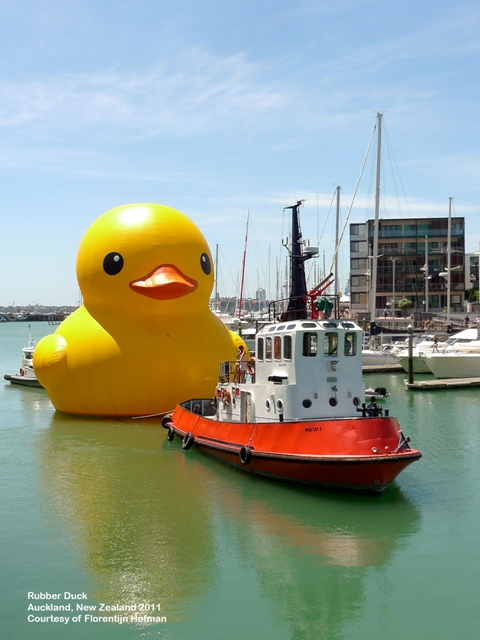
\includegraphics[width=0.95\textwidth]{img/rubberduck.jpg}
  \caption{caption}
  \label{fig:label}
\end{figure}


% subsection Template (end)


